This chapter describes specific implementation details of IDDR system.

\section{Overview} 
We implemented the IDDR system based on the Linux kernel, version 3.5.0 and
Xen version 4.2.1. The application domain and the driver domain run the same kernel
binary. Table~\ref{tab:base} summarizes our implementation efforts in
terms of the number of lines of code.

\begin{table}
\caption{Implementation efforts in terms of number of lines of code.}
\begin{center}
\begin{tabular}{lll}
  \hline
  \label{tab:base}
  Component & Interrupt based IDDR & Spinning based IDDR \\
  \hline
  Linux Kernel & 6 & 6\\
  Xen & 252 & 252\\
  Front-end Driver & 611 & 712\\
  Back-end Driver & 692 & 752\\
  \hline 
  Total & 1561 & 1722\\
  \hline
\end{tabular}
\end{center}
\end{table}

The IDDR system implementation did not require any changes to the device
driver code. However, we did make a small number of changes to the Xen
and Linux kernel.

Figure~\ref{fig:Implementation overview} shows the implementation overview of 
the spinning based IDDR system.

\begin{figure}[!ht]
\centering
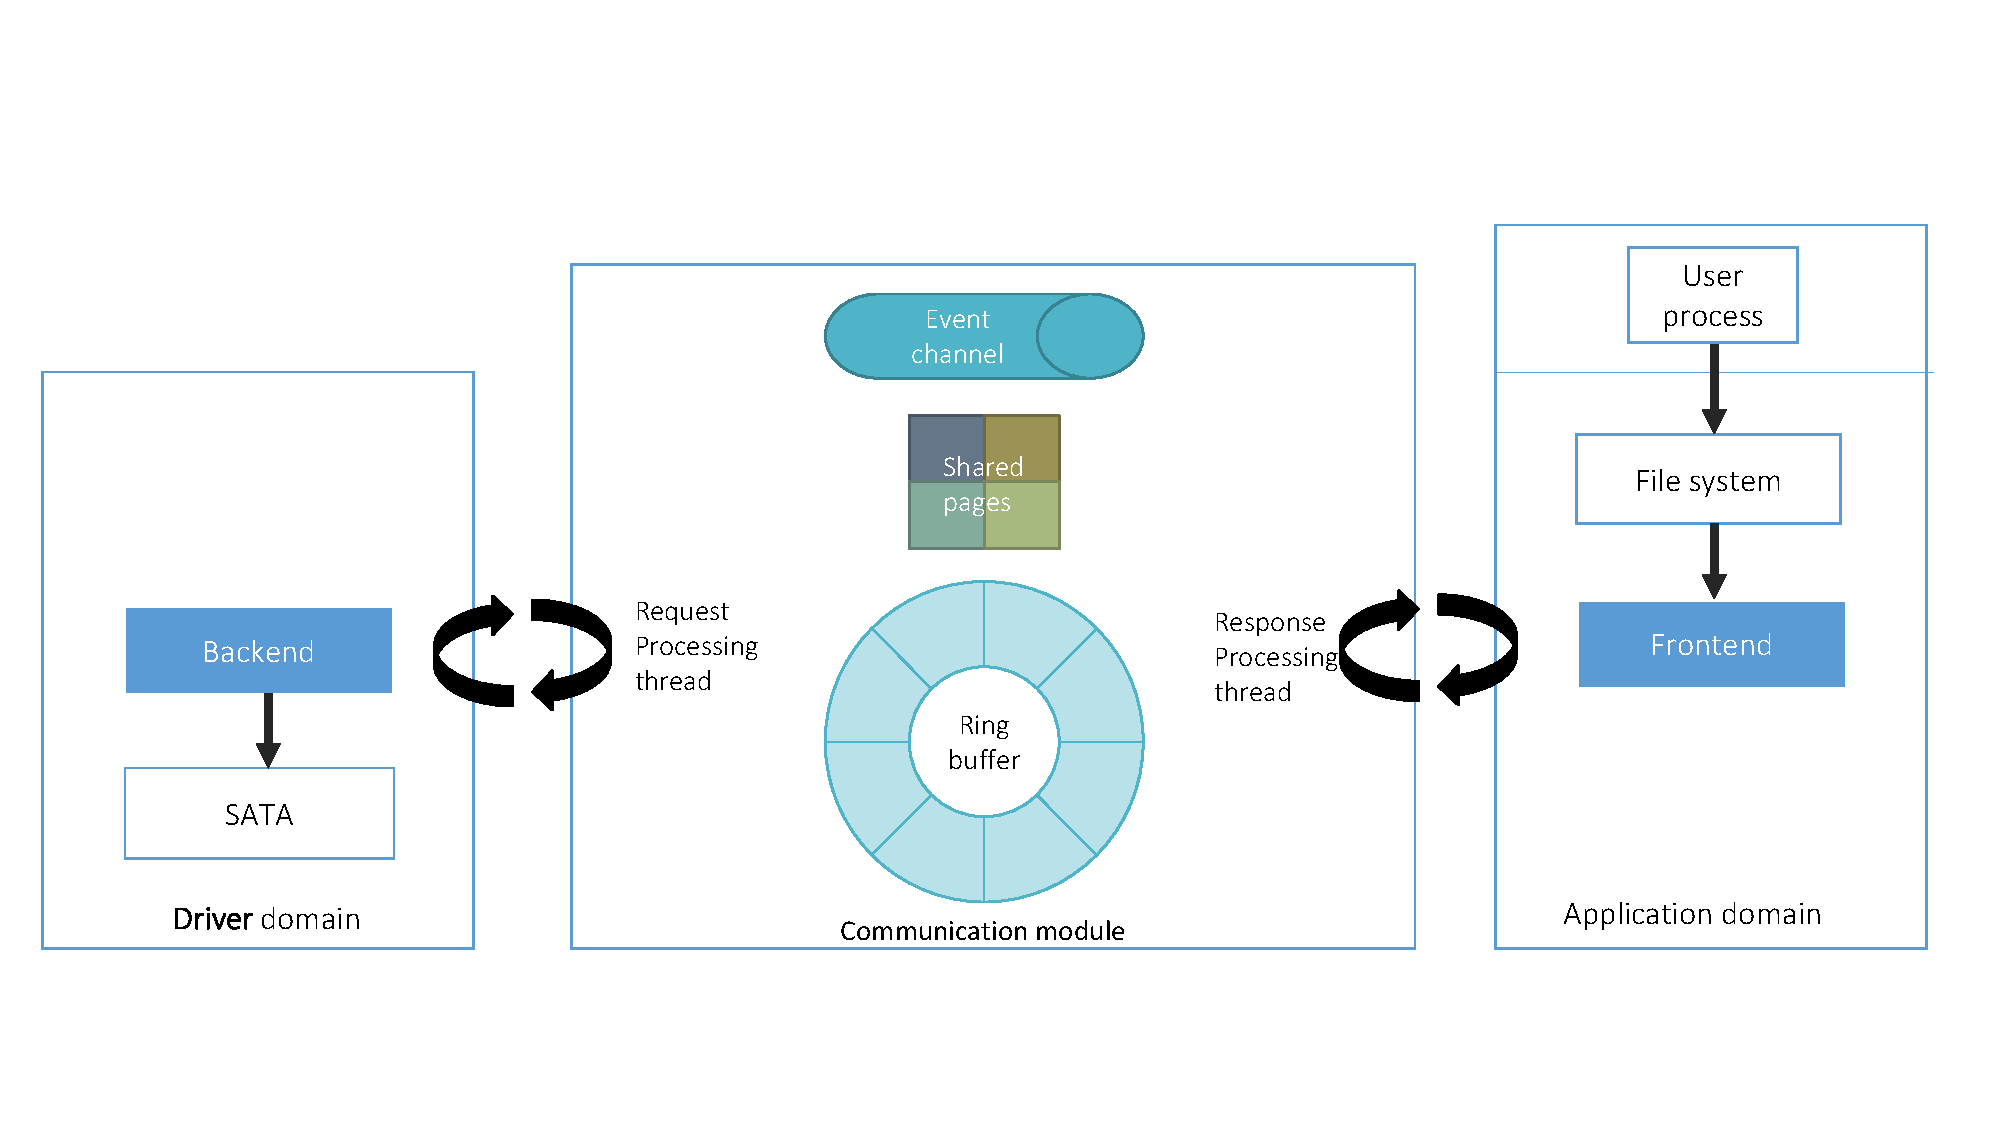
\includegraphics[scale=.5]{impl_overview_new}
\caption{Implementation overview of spinning based IDDR system}
\label{fig:Implementation overview}
\end{figure}

\section{Communication Module}
This section describes the implementation details of the communication
module of interrupt based IDDR system and spinning based IDDR system.

\subsection*{Interrupt based IDDR system}
As Section~\ref{sub:communicationmodule} describes, the role of the communication module in interrupt based IDDR system is to:
\begin{enumerate} 
\item Share requests and responses between the driver domain and the application domain
\item Share the data associated with read/write requests/responses
\item Notify the domain upon the availability of requests and responses 
\end{enumerate}
\paragraph{Shared Request and Response Queue:}
In order to implement the first role of the communication module, we
use the ring buffer mechanism provided by Xen. A ring buffer is a shared
I/O ring, which is explained in Section~\ref{subsec:io rings}. We divide
the ring buffer into the front ring and the back ring. The IDDR system
uses the front ring as the shared request queue and the back ring as
the shared response queue. The front ring shares requests and is called
as \textit{shared request queue}. The back ring shares responses and is
called as \textit{shared response queue}.

The IDDR system allocates the ring buffer in the initialization stage
of the communication module and initializes the ring buffer in the
application domain. Whenever the frontend driver receives a request from
an application in the application domain, the frontend driver removes the
request from the device driver queue and submits it to the communication
module. The communication module checks for a free space in the shared
request queue, and if available, it allocates the space for the new
request. After batching requests together, the communication module
pushes all requests to the shared request queue.

\paragraph{Shared Memory for Read/Write Data:}
We use the ring buffer only to share requests and responses. In order
to share data associated with read/write requests/responses we use
shared pages.

As explained in Section~\ref{subsec:sharedpages}, a grant table is used
for sharing memory between domains. We use a grant table to share memory
between the application domain and the driver domain.

\paragraph{Event Notification:}
We create a new event channel in the initialization stage of the
communication module in the application domain and connect to the same
event channel in the initialization stage of the communication module
in the driver domain. We attach an interrupt handle routine for the
event channel in both the application and driver domain. The interrupt
handler routine in the application domain reads responses from the shared
response queue and forwards them to the frontend driver. The interrupt
handler routine in the driver domain reads requests from the shared
request queue and forwards them to the backend driver.

\subsection*{Spinning Based IDDR System}
This section describes the communication module in 3 parts:

\paragraph{Shared Request and Response Queue:}
Similar to the interrupt based IDDR system, the communication module
uses a ring buffer as the shared request and response queue.

\paragraph{Shared Memory for Read/Write Data:}
Similar to interrupt based IDDR system, the communication module uses a
grant table to share an allocated memory between the application domain
and the driver domain.

\paragraph{Threads and Event Notification:}
In order to improve the performance of the IDDR system, we implement the
communication module where a thread in the frontend driver spins for the
availability of responses, and a thread in the backend driver spins for
the availability of requests. In case of unavailability of requests and
responses, both threads go to sleep.

The spinning based IDDR system uses an event channel to wake the read
request thread sleeping in the application domain. The wake up signal
is sent in the form of an event channel notification from the driver
domain to the application domain. Similarly, to wake the read response
thread sleeping in the driver domain, an event channel notification is
sent from the application domain to the driver domain.

\begin{itemize}
\item \textbf{Read response thread in the application domain:} 
In the spinning based IDDR system we create a kernel thread called the \textit{read
response thread} during an initialization stage of the communication
module in the application domain. The \textit{read response thread} spins
to check if responses are available in the shared response queue. If a
response is available, it reads the response from the shared response
queue. However, if a response is not available in the shared response
queue, after spinning for some time the thread goes into a sleep state. We
maintain the status of the thread as \texttt{SLEEPING} or \texttt{RUNNING}
in the shared data structure. We use an atomic variable to save the
state of the thread, avoiding race conditions.

Obviously, a thread shouldn't sleep unless it is assured that somebody else, somewhere, will wake it up. The code doing the waking up must also be able to identify the thread to be able to do its job. We use a Linux data structure called \texttt{wait queue} to find the sleeping thread. Wait queue is a list of threads, all waiting for a specific event\cite{Galvin, Bovet:2005:ULK:1077084}. We initialize the wait queue for the read response thread during an initialization stage of the communication module in the application domain. The read response thread sleeps in the wait queue, waiting for a flag denoting the availability of the response to be set. The communication module in the driver domain checks the status of the read response thread after pushing responses on the shared response queue. If the status is \texttt{SLEEPING} then it sends a software interrupt through the event channel.

Similar to interrupt based IDDR system, we create a new event channel in
the initialization stage of the communication module in the application
domain. We attach an interrupt handler routine for the event channel
in the application domain. In the interrupt handler, the communication
module wakes up the read response thread if it is sleeping.

\item \textbf{Read request thread in the driver domain:}
In spinning based IDDR system, we create a kernel thread during
an initialization stage of the communication module in the driver
domain. This new kernel thread is called the \textit{read request
thread}. The \textit{read request thread} spins to check if requests are
available in the shared request queue. If a request is available, it reads
the request from the shared request queue. However, if a request is not
available in the shared request queue, the thread goes into a sleep state
after spinning for some time (adaptive spinning). Similar to the read
response thread, we maintain the status of the thread as \texttt{SLEEPING}
or \texttt{RUNNING} as a atomic variable in the shared data structure.

We initialize a wait queue for the read request thread during
an initialization stage of the communication module in the driver
domain. The read request thread sleeps in the wait queue, waiting for a
flag denoting availability of the request to be set. The communication
module in the application domain checks the status of the read request
thread after pushing requests on the shared request queue. If the status
is \texttt{SLEEPING} then it sends a software interrupt through the
event channel.

Similar to interrupt based IDDR system, the driver domain connects to the
event channel created by the application domain in the initialization
stage of the communication module. We attach an interrupt handler
routine for the event channel in the application domain. In the interrupt
handler, the communication module wakes up the read request thread if
it is sleeping.  
\end{itemize}

\section{Application Domain}

Application domain is the domain running user applications and the Linux
kernel. In a Linux system, usually a user process sends the read write
request to a file system, which sends the read and write request to
the block device driver. The block device driver serves the request and
sends back a response to the file system, which then sends the response
to the user process.

In the IDDR system implementation, a block device runs separately in
the driver domain. When a user process sends a request to a file system,
the file system needs to forward the request to the driver domain. Like
explained in Section~\ref{subsec:frontend}, in the IDDR system, a piece
of code called the frontend driver forwards the request to the driver
domain running the block device driver.

\subsection*{Interrupt based IDDR System}
The core responsibility of the frontend driver in interrupt based IDDR system is to:
\begin{enumerate}
\item Provide an interface which appears as a block device to the upper layer in the stack
\item Accept a request from the upper layer
\item Create a corresponding new request which can be understood by the driver domain
\item End the request after reading the response
\end{enumerate}

Implementation details of the frontend driver can be split into 3 stages: 
\begin{enumerate}
\item Initialization
\item Submit request to the communication module
\item End request
\end{enumerate}

\paragraph{Initialization}
During the initialization, the frontend driver creates a separate
interface for each block device. The interface for each block device is
associated with a device driver queue. Read and write requests issued
on the interface get queued in this device driver queue.

\paragraph{Dequeue and Submit Request:}
The frontend driver removes the request submitted to the driver
interface and converts the request into a request structure, which is
understood by the backend driver. The new request structure points to
the shared memory allocated for the read/write data by the communication
module. The frontend driver then forwards the newly created request
to the communication module, which also shares the request with the
backend driver.

\paragraph{End Request:}
We maintain a shadow table of all requests which were received in the
device driver queue. The shadow table is a table which contains an entry
of all the requests received. We implement the shadow table as a circular
array of the requests. We maintain an ID for each request. The backend
driver copies this ID into the corresponding response. The ID is used
for mapping the response to the request in the shadow table. When a
response is read by the communication module, it forwards the response
to the frontend driver. The frontend driver searches the corresponding
request in the shadow table, and ends it.

\subsection*{Spinning Based IDDR System}
The core responsibility of the frontend driver in spinning based IDDR system is to:
\begin{enumerate}
\item Provide an interface for each block device
\item Accept a request from the upper layer
\item Create a corresponding new request which can be understood by the driver domain
\item Spin for a short time while waiting for the response
\item End the request
\end{enumerate}

Implementation details of the frontend driver is split into 4 stages:
\begin{enumerate}
\item Initialization
\item Submit request to the communication module
\end{enumerate}

\paragraph{Initialization:}
Similar to interrupt based IDDR system, during the initialization process the frontend driver creates an interface for each block device.

\paragraph{Dequeue and Submit Request:}
Similar to interrupt based IDDR system, the frontend driver removes the
request submitted to the driver interface and converts it into the request
structure with a data pointer pointing to the shared memory. The frontend
driver then forwards the newly created request to the communication
module, which also shares the request with the backend driver.

\section{Driver Domain}
The IDDR system runs a block device driver in the driver domain. Like
explained in Section~\ref{subsec:backend}, a piece of code called the
backend driver runs in the driver domain, which accepts requests from
the application domain and forwards requests to the device driver. Upon
receiving a response from the device driver, the backend driver sends
back the response to the communication module.

\subsection*{Backend Driver}
The role of the backend driver in the IDDR system is to:
\begin{enumerate}
\item Read a request through the communication module and convert it to a bio request
\item Accept a response from the block device driver
\item Forward the response to the communication module
\end{enumerate}

Implementation details of the backend driver can be split into 2 stages. 
\begin{enumerate}
\item Convert a request to the bio request. 
\item Make a response.
\end{enumerate}

\subsubsection*{Convert a Request to Bio}
\label{subsec:createbio}
The backend driver converts a request that is shared through the
communication module into a bio request, so that the block device
understands the request. In order to make the bio request, pages from
the shared memory are mapped and inserted into the bio structure and
required information is copied from the shared request into the bio
structure. At the end, the newly created bio request is sent to the
lower layer for execution. Once the bio request execution is completed,
the system calls a callback function.

\subsubsection*{Make a Response and Enqueue}
Irrespective of the success or failure of execution of a bio request,
the backend driver makes a response in the callback function. In this
callback function, the result of the bio execution and a request ID is
copied into a newly allocated response structure. The request ID is used
as an index in the shadow table to map a response and a request. The
communication module pushes the response into the shared response queue.

